

En este capítulo se comentará el diseño de la aplicación de manera superficial, la arquitectura general, el modelo de datos y también aspectos más concretos del diseño del servidor.


\section{Esquema general de la arquitectura}

La aplicación que estamos desarrollando seguirá la arquitectura
en tres capas. Este patrón arquitectónico cliente/servidor se diferencian tres
capas, una capa de interface de usuario , una capa de persistencia
y una capa intermedia llamada de servicios que permite la llamada de forma remota a la capa modelo(capa que contiene la lógica) por parte del cliente. Este esquema esta compuesto por:




\begin{figure}[H]
		\centering
		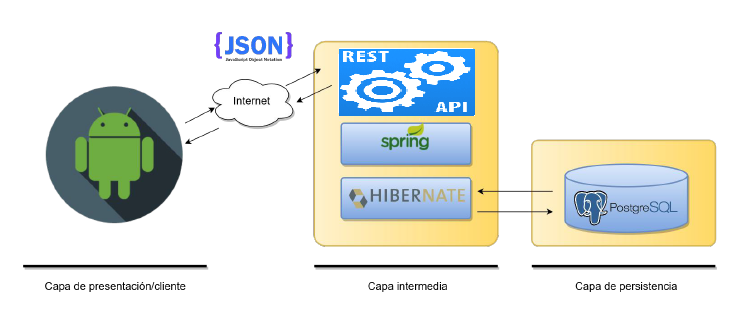
\includegraphics[width=0.75\textwidth] {arquitectura.png}
		\caption{Esquema general de la arquitectura del sistema }
	\end{figure}


\begin{itemize}
\item \textbf{Capa de presentación/cliente}:\\
Capa que  nos proporciona la información relacionada con los servicios que puede invocar el cliente. Es la encargada de comunicarse con las otras capas para guardar la información de cada usuario.En si es la capa con la que va a interactuar el usuario cada vez trabaje con esta aplicación.
\item \textbf{Capa intermedia:}\\
Esta capa es la encargada de enlazar la capa de persistencia con la capa de presentación/cliente. Lo que hace es recoger los datos que provienen de la base de datos, necesarios para satisfacer el servicio invocado y enviárselos al cliente.

\item \textbf{Capa de persistencia:}\\
Esta capa es la encargada de almacenar los datos del sistemas en la base de datos, además contiene todos los mecanismos de acceso a datos necesarios para poder hacer persistentes los datos.
 Esta capa debe ofrecer una interface que ayude a la comunicación con la capa intermedia, de manera que se abstraiga de la tecnología usada en el sistema de almacenamiento y no crea una dependencia con ella. Esta abstracción permitirá hacer cambios o actualizaciones en la tecnología sin afectar a otras capas con las que pudiera interaccionar en un futuro.\\
 


\end{itemize}
Un vez comentada la arquitectura general del sistema, pasaremos a comentar la capa intermedia un poco más a fondo ya que en ciertas ocasiones, la capa intermedia puede estar compuesta de N-capas(Arquitectura en N-capas). Ésta es una de esas ocasiones.

Los servidores que siguen el modelo Modelo-Vista-Controlador consiguen separar los datos de la  aplicación, la lógica de negocio  y el envío  de información por la red.
Ésta separación ayuda al desarrollo de la aplicación tanto a la hora de crear la como a la hora de hacer su mantenimiento ya que marca al desarrollador a colocar el código en una capa concreta. \\


Los componentes capas que componen al patrón MVC son:

\begin{itemize}
\item \textbf{Modelo:}\\
Está compuesta por clases que tienen acceso a los datos ofreciendo unos métodos que pueden ser usados de manera sencilla por las capas superiores. Éstos métodos son los encargados de acceder a la base de datos y proporcionar los datos persistentes.



\item \textbf{Vista:}\\

Esta formada por el interfaz donde se realizan las llamadas entre el servicio web, peticiones HTTP en las que la información va en formato JSON, y la aplicación cliente.

\item \textbf{Controlador:}\\
Esta capa será la encargada de implementar la lógica del interface llamando a las operaciones que ofrece el modelo y seleccionando la vista asociada a cada petición.



\end{itemize}


\section{Modelo de datos}

\section{Servidor}

Para que pudiera haber una comunicación entre la aplicación del cliente y la capa de persistencia hemos desarrollado una solución que se desplegará a través de un interface, al que se podrá acceder de manera remota y que permitirá tener acceso a las funcionalidades de la capa persistente.

La solución mencionada anteriormente será una aplicación, en java, que  usará Spring ya que facilita la creación de aplicaciones de forma cómoda y rápida.\\

Durante el desarrollo  de este proyecto el servidor ha sido desplegado en un proveedor de servidores virtuales llamado 
  DigitalOcean,ya que ofrece distintos lugares donde poder ubicar lo hemos decidido hacerlo en uno concreto de Alemania para que el ping fuera mas cercano y rápido.
\begin{figure}[H]
		\centering
		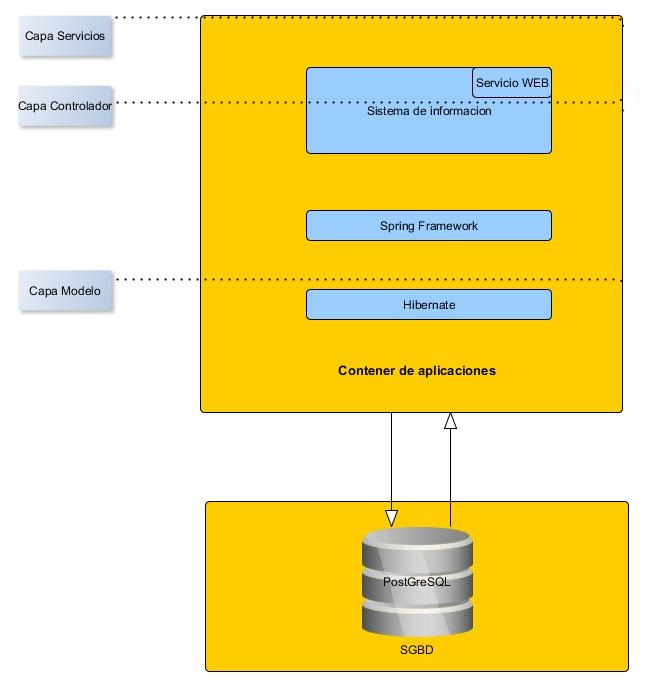
\includegraphics[width=0.75\textwidth] {arquitectura-servidor.jpg}
		\caption{Arquitectura del servidor }
	\end{figure}


\subsection{Servizo web}
A comunicacion farase a traves do paradigma Rest que e un estilo arquitectonico para
construr aplicacions distribudas inspirado nas caractersticas da web e que emprega
directamente HTTP para obtencion de datos. A traves das seguintes peticions HTTP
poderemos acceder os distintos recursos.


\begin{itemize}
\item Os metodos de acceso especican a accion que se quere realizar sobre un recurso. Desta
forma o usar GET solicitarase unha representacion do recurso pedido. PUT crea
unha nova representacion dun recurso e POST modifcaa. Tamen existe o metodo
DELETE que elimina o recurso especicado.
\item Dependendo do metodo que se empregue a ruta sobre a que se fai a peticion HTTP
e distinta. Tanto POST como DELETE realzanse sobre recursos especco, polo tanto
a ruta parecerase a : . PUT empregase sobre recursos
coleccion /recursos. O metodo GET pode ser usando tanto en recursos coleccion
como individuais.


\end{itemize}

\subsection{Organizacion dos paquetes}

\subsection{Transmision de Informacion}

\subsection{Xestion das clases persistentes}

\section{Aplicación Móvil}